\subsection{对实际工作负载的评估}
\label{subsec:real-world}

我们使用真实世界的工作负载(包含重复)评估 \sysname。我们在评估中考虑了两个真实世界的数据集。
\begin{itemize}[leftmargin=*]
\item 第一个数据集,称为 \textit{ FSL},包含来自文件系统和存储实验室 (FSL) \cite{fsl,sun16} 的共享文件系统的用户主目录的备份快照。每个快照列出了平均块大小为 8\,KB 的块的 48 位指纹。我们选择了 2013 年 1 月 22 日至 6 月 17 日的所有快照(在 \texttt{fslhomes} 下),总共覆盖了 56.2\,TB 的预去重数据。重复数据删除后数据集减少到 431.9\,GB(即 133.2$\times$ 的重复数据删除率)。
\item 第二个数据集,称为 \textit{ MS},包含来自 Microsoft \cite{meyer11} 的 Windows 文件系统快照。每个快照列出了平均块大小为 8\,KB 的块的 40 位指纹。我们从原来的 857 个快照中抽取了 140 个快照,每个快照的大小约为 100GB。我们的数据集包含 14.4 TB 的预去重数据。重复数据删除后,它减少到 2.4\,TB(即 6$\times$ 的重复数据删除率)。
\end{itemize}



\paragraph{Exp\#8 (Trace-driven performance).} 我们对\sysname 的上传和下载性能进行了trace-driven 评估。我们从 FSL 和 MS 中分别选择了 10 个快照,如下所示。对于 FSL,我们选择来自同一用户的快照具有较高的跨快照冗余;对于 MS,我们选择具有最多快照内冗余的快照。选择的 FSL 和 MS 快照分别采用 1.3\,TB 和 1.0\,TB 的预去重数据。由于我们的快照只包含没有实际数据的指纹,我们通过重复将其指纹写入备用块直到达到指定的块大小来重构每个明文块,因此相同(不同)指纹返回相同(不同)块。我们使用单个客户端一张一张地上传快照,然后以相同的上传顺序下载它们。我们将 \sysname 与 PlainDedup (Exp\#4) 进行比较。

\begin{figure}[t]
  \centering
  \begin{tabular}{@{\ }c@{\ }c}
  %\begin{tabular}{@{\ }p{1.68in}p{1.68in}}
  \multicolumn{2}{c}{
\includegraphics[width=\textwidth]{pic/sgxdedup/expb2_trace_legend.pdf}} \\
  \hspace{-0.1in}
  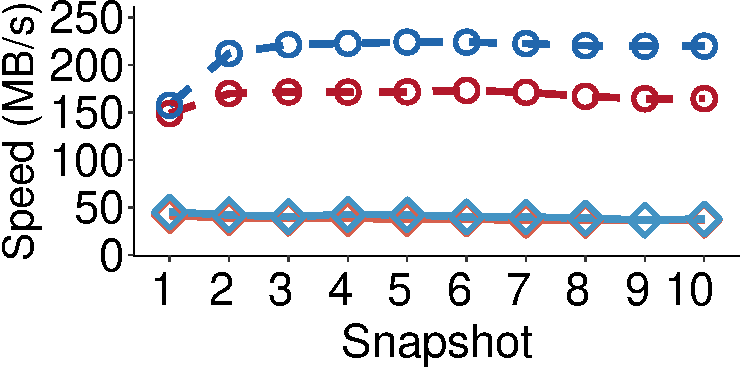
\includegraphics[width=0.48\textwidth]{pic/sgxdedup/expb2_trace_fsl_plain_sgx.pdf} &
  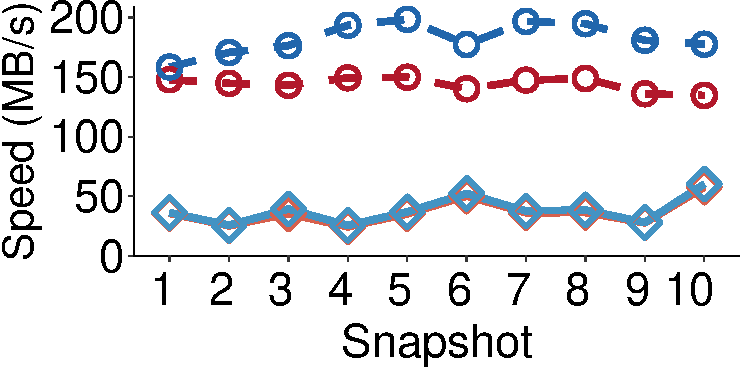
\includegraphics[width=0.48\textwidth]{pic/sgxdedup/expb2_trace_ms_plain_sgx.pdf}
  \vspace{-3pt}\\
  \mbox{\small (a) FSL dataset} &
  \mbox{\small (b) MS dataset}
  \end{tabular}
  \vspace{-6pt}
  \caption{(Exp\#8) Trace-driven upload and download performance.}
  \label{fig:tracePerformance}
\end{figure}

图~\ref{fig:tracePerformance}(a) 显示了跨 FSL 快照的上传和下载速度。 \sysname 和 PlainDedup 都实现了很高的上传速度,尤其是在第一个快照(例如 148.8\,MB/s \sysname 为 ,PlainDedup 为 157.5\,MB/s)。原因是 FSL 数据集跨快照的冗余度很高,两个系统都可以为后续快照上传较少的数据。与 PlainDedup 相比,\sysname 平均会导致上传性能下降 22.0\%。请注意,在我们使用合成工作负载的性能评估 (Exp\#4) 中,开销略大于 (17.5-21.4\%)。原因是现在在跟踪驱动评估中禁用了分块,\sysname 的瓶颈切换到 PoW(参见表~\ref{tab:system-breakdown}),而 PlainDedup 的瓶颈是指纹。 \sysname 的下载速度从 41.3\,MB/s 下降到 36.4\,MB/s,PlainDedup 的下载速度从 45.0\,MB/s 下降到 37.9\,MB/s,主要是由于块碎片 \cite{lillibridge13} .我们可以通过重写和缓存 \cite{lillibridge13,cao18} 来减轻块碎片。

图~\ref{fig:tracePerformance}(b) 显示了跨 MS 快照的上传和下载速度。这两个系统的上传速度都低于 FSL 数据集,因为 MS 数据集有更多的非重复块(例如,MS 为 28.7\,M 而 FSL 为 18.3\,M)并加重了指纹索引的访问开销。与 PlainDedup 相比,\sysname 平均会导致 21\% 的上传速度下降。请注意,下载速度会波动(例如,\sysname 为 24.3-57.5\,MB/s,PlainDedup 为 25.6-60.3\,MB/s),因为某些 MS 快照具有更多非重复块,并且可能存储在可以通过顺序读取快速访问的连续区域(即更少的块碎片 \cite{lillibridge13})。

\paragraph{Exp\#9(节省带宽)。} 我们评估 \sysname 的带宽效率。我们考虑使用基于源的重复数据删除(即客户端执行重复数据删除并仅将非重复的密文块上传到云)和基于目标的重复数据删除(即客户端上传所有密文块到云,对收到的密文块执行重复数据删除):(i)\textit{ 两阶段重复数据删除} \cite{li15},对单个用户应用基于源的重复数据删除,然后跨用户应用基于目标的重复数据删除; (ii) \textit{ 随机阈值重复数据删除} \cite{harnik10},它基于随机选择的阈值执行基于源的重复数据删除或基于目标的重复数据删除。我们在随机阈值重复数据删除中选择阈值的上限和下限分别为 20 和 2,如 \cite{harnik10}。对于FSL,我们聚合不同用户的当天快照,并将每个聚合快照按照创建时间的顺序添加到存储中。对于 MS,我们根据其快照 ID 添加每个快照(我们假设每个 MS 快照来自不同的用户)。我们将 \textit{ 带宽节省} 衡量为与预去重数据相比传输中数据减少的比例。在这里,我们不考虑元数据导致的带宽开销。

图~\ref{fig:uploadTraffic} 显示了上传每个快照后的累积带宽节省。上传所有快照后,\sysname 在 FSL 和 MS 中分别实现了 99.2\% 和 83.2\% 的带宽节省。由于 \sysname 执行基于源的重复数据删除,因此其带宽节省也转化为存储节省。两阶段重复数据删除与 FSL 中的 \sysname 节省的带宽几乎相同,因为 FSL 数据集包含大量用户内冗余。另一方面,在 MS 中,两级重复数据删除仅节省了 47.9\% 的带宽(比 \sysname 少了 35.3\% 的绝对差异)。随机阈值重复数据删除具有不同的带宽节省,在 MS 中节省了 48.5\%,但在 FSL 中只有 7.8\%(小于 \sysname,绝对差异分别为 34.7\% 和 91.4\%)。

\begin{figure}[t]
\centering
\begin{tabular}{@{\ }c@{\ }c}
%\begin{tabular}{@{\ }p{1.68in}p{1.68in}}
\multicolumn{2}{c}{
\includegraphics[width=\textwidth]{pic/sgxdedup/upload_traffic_legend.pdf}} \\
\hspace{-0.1in}
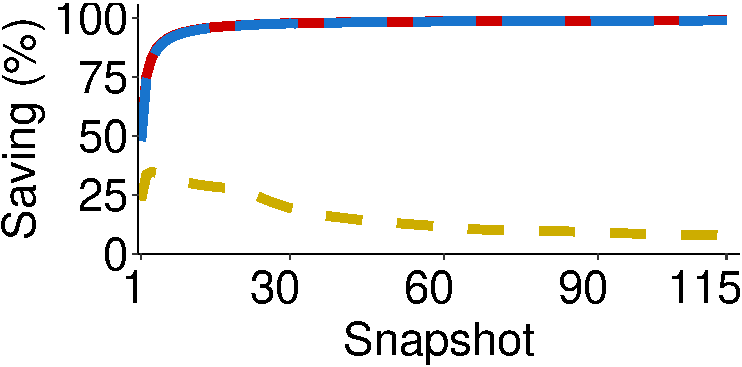
\includegraphics[width=0.48\textwidth]{pic/sgxdedup/upload_traffic_fsl.pdf} &
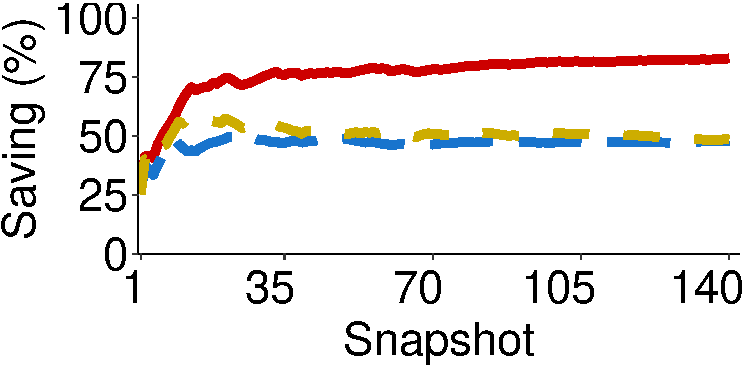
\includegraphics[width=0.48\textwidth]{pic/sgxdedup/upload_traffic_ms.pdf}
\vspace{-3pt}\\ 
\mbox{\small (a) FSL dataset} &
\mbox{\small (b) MS dataset}
\end{tabular}
\vspace{-6pt}
\caption{(Exp\#9) Cumulative bandwidth savings after each snapshot is stored.}
\label{fig:uploadTraffic}
\end{figure}

